\documentclass[11pt, leqno]{scrartcl}
\usepackage{polski}
\usepackage[polish]{babel}

\usepackage{graphicx, float, caption, subcaption}
\usepackage{tabularx, multirow, hyperref, enumitem}
\usepackage{listings, xcolor}
\usepackage{amsmath, amssymb}
\usepackage{algorithm}
\usepackage{algpseudocode}
%\usepackage{minted}

\definecolor{md-black}{rgb}{0.12, 0.12, 0.12}
\definecolor{md-teal}{rgb}{0.38, 0.79, 0.69}
\definecolor{md-mauve}{rgb}{0.76, 0.52, 0.75}
\definecolor{md-yellow}{rgb}{0.86, 0.86, 0.67}
\definecolor{md-green}{rgb}{0.13, 0.55, 0.13}
\definecolor{md-red}{rgb}{0.82, 0.10, 0.14}
\definecolor{md-gray}{rgb}{0.44, 0.46, 0.51}

\hypersetup{
    colorlinks=true,
    linkcolor=black,
    urlcolor=black,
    citecolor=black
}

\lstset{
    language=Python,
    basicstyle=\color{md-teal}\ttfamily,
    keywordstyle=\color{md-mauve},
    commentstyle=\color{md-green},
    stringstyle=\color{md-red},
    numbers=left,
    numberstyle=\small\color{md-gray}\ttfamily,
    stepnumber=1,
    numbersep=5pt,
    backgroundcolor=\color{md-black},
    showspaces=false,
    showstringspaces=false,
    showtabs=false,
    frame=none,
    tabsize=4,
    captionpos=b,
    breaklines=true,
    breakatwhitespace=false,
    escapeinside={\%*}{*)},
    numbersep=-10pt,
    morekeywords={as},
    classoffset=1,
    morekeywords={curve_fit},
    keywordstyle=\color{md-yellow},
    classoffset=0
}

\graphicspath{{../images/}}

\title{IV zestaw zadań - Mnożenie macierzy hierarchicznych}
\author{Kacper Kozubowski, Mateusz Podmokły \\ III
    rok Informatyka WI}
\date{11 grudnia 2024}

\begin{document}
    \maketitle
    \section{Treść zadania}
    Należy wygenerować macierz o rozmiarze $2^{3k}=2^k \cdot 2^k
    \cdot 2^k$ dla $k \in \{2,3,4\}$ o strukturze opisującej
    topologię trójwymiarowej siatki zbudowanej z elementów
    sześciennych. Następnie wykonać polecenia:
    \begin{enumerate}
        \item użyć rekurencyjną procedurę kompresji macierzy
            z Zadania 3,
        \item narysować macierz skompresowaną używając funkcji
            z Zadania 3,
        \item przemnożyć macierz skompresowaną przez wektor,
        \item przemnożyć macierz skompresowaną przez samą siebie.
    \end{enumerate}

    \section{Specyfikacja użytego środowiska}
    Specyfikacja:
    \begin{itemize}
        \item Środowisko: Jupyter Notebook,
        \item Język programowania: Python,
        \item System operacyjny: Microsoft Windows 11,
        \item Architektura systemu: x64.
    \end{itemize}

    \section{Działanie algorytmów}
    \subsection{Wykorzystane biblioteki}
    W realizacji rozwiązania wykorzystane zostały następujące
    biblioteki:
    \begin{lstlisting}
    import numpy as np
    import cv2
    import matplotlib.pyplot as plt
    import matplotlib.patches as patches
    \end{lstlisting}

    \subsection{Kod funkcji}
    W zadaniu wykorzystane zostały funkcje \texttt{truncated\_SVD},
    \texttt{compress\_matrix}, \\
    \texttt{create\_tree} oraz klasa \texttt{Node} z Zadania 3.
    \begin{figure}[H]
        \centering
        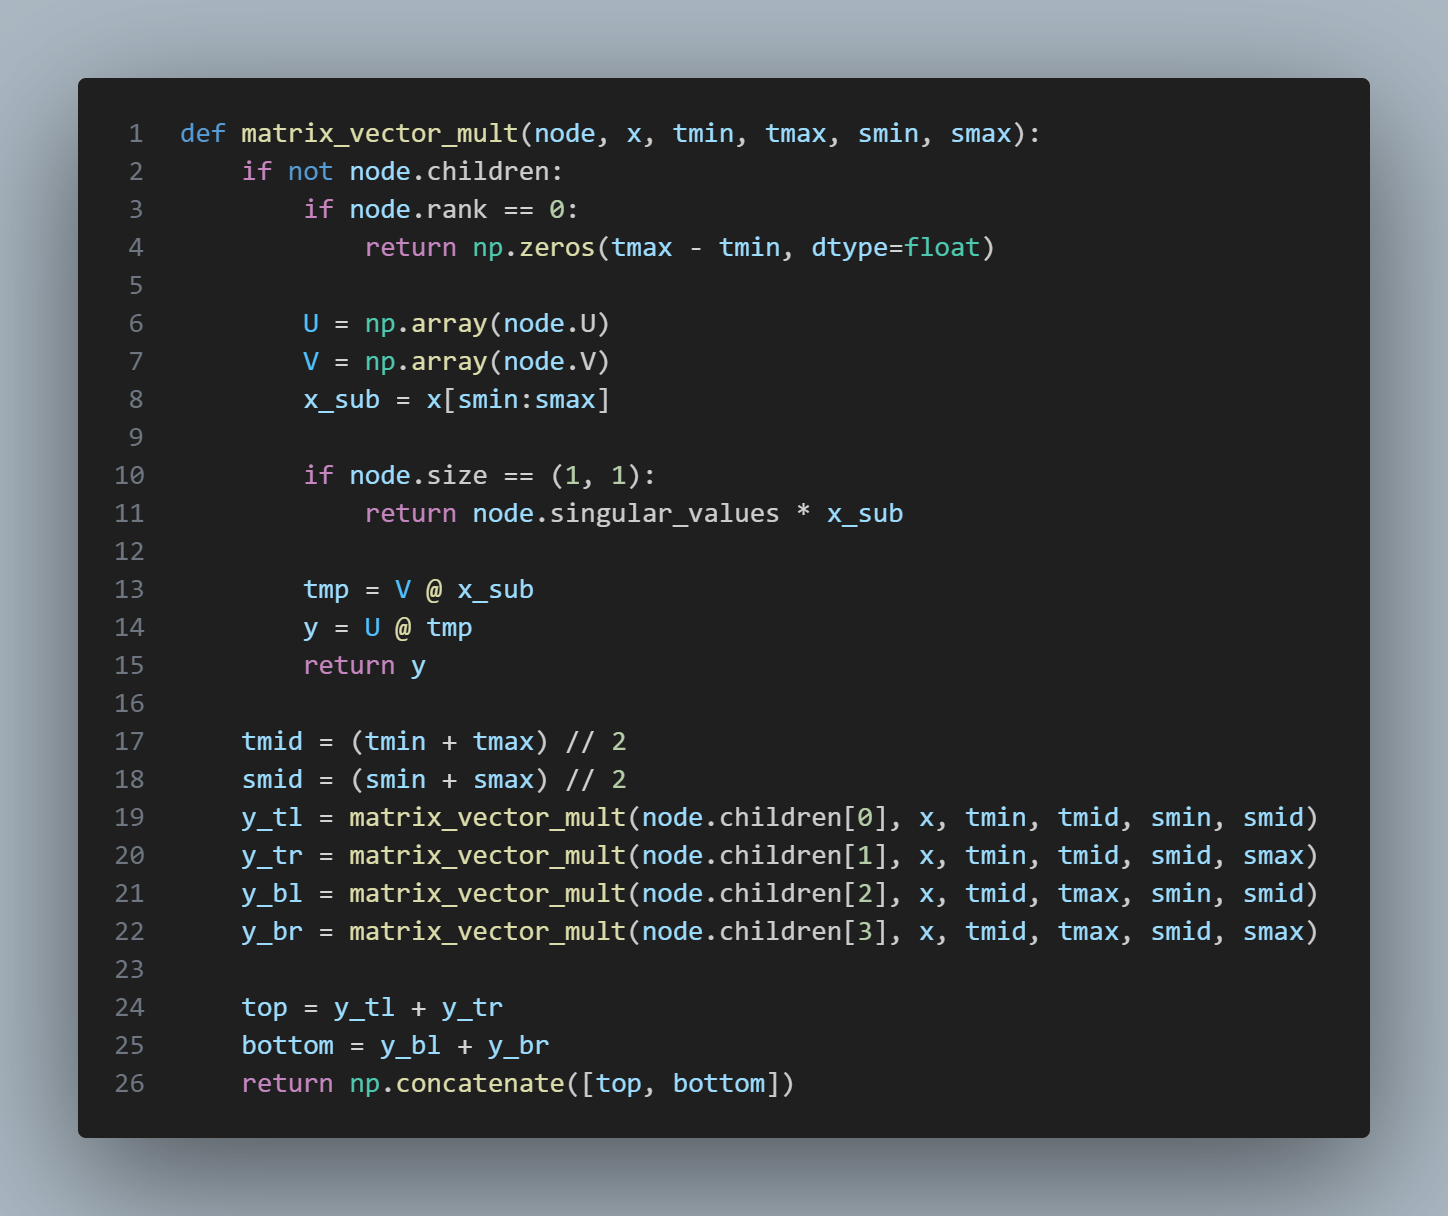
\includegraphics[width=1\linewidth]{matrix_vector.png}
        \caption{Mnożenie macierzy przez wektor.}
    \end{figure}
    \begin{figure}[H]
        \centering
        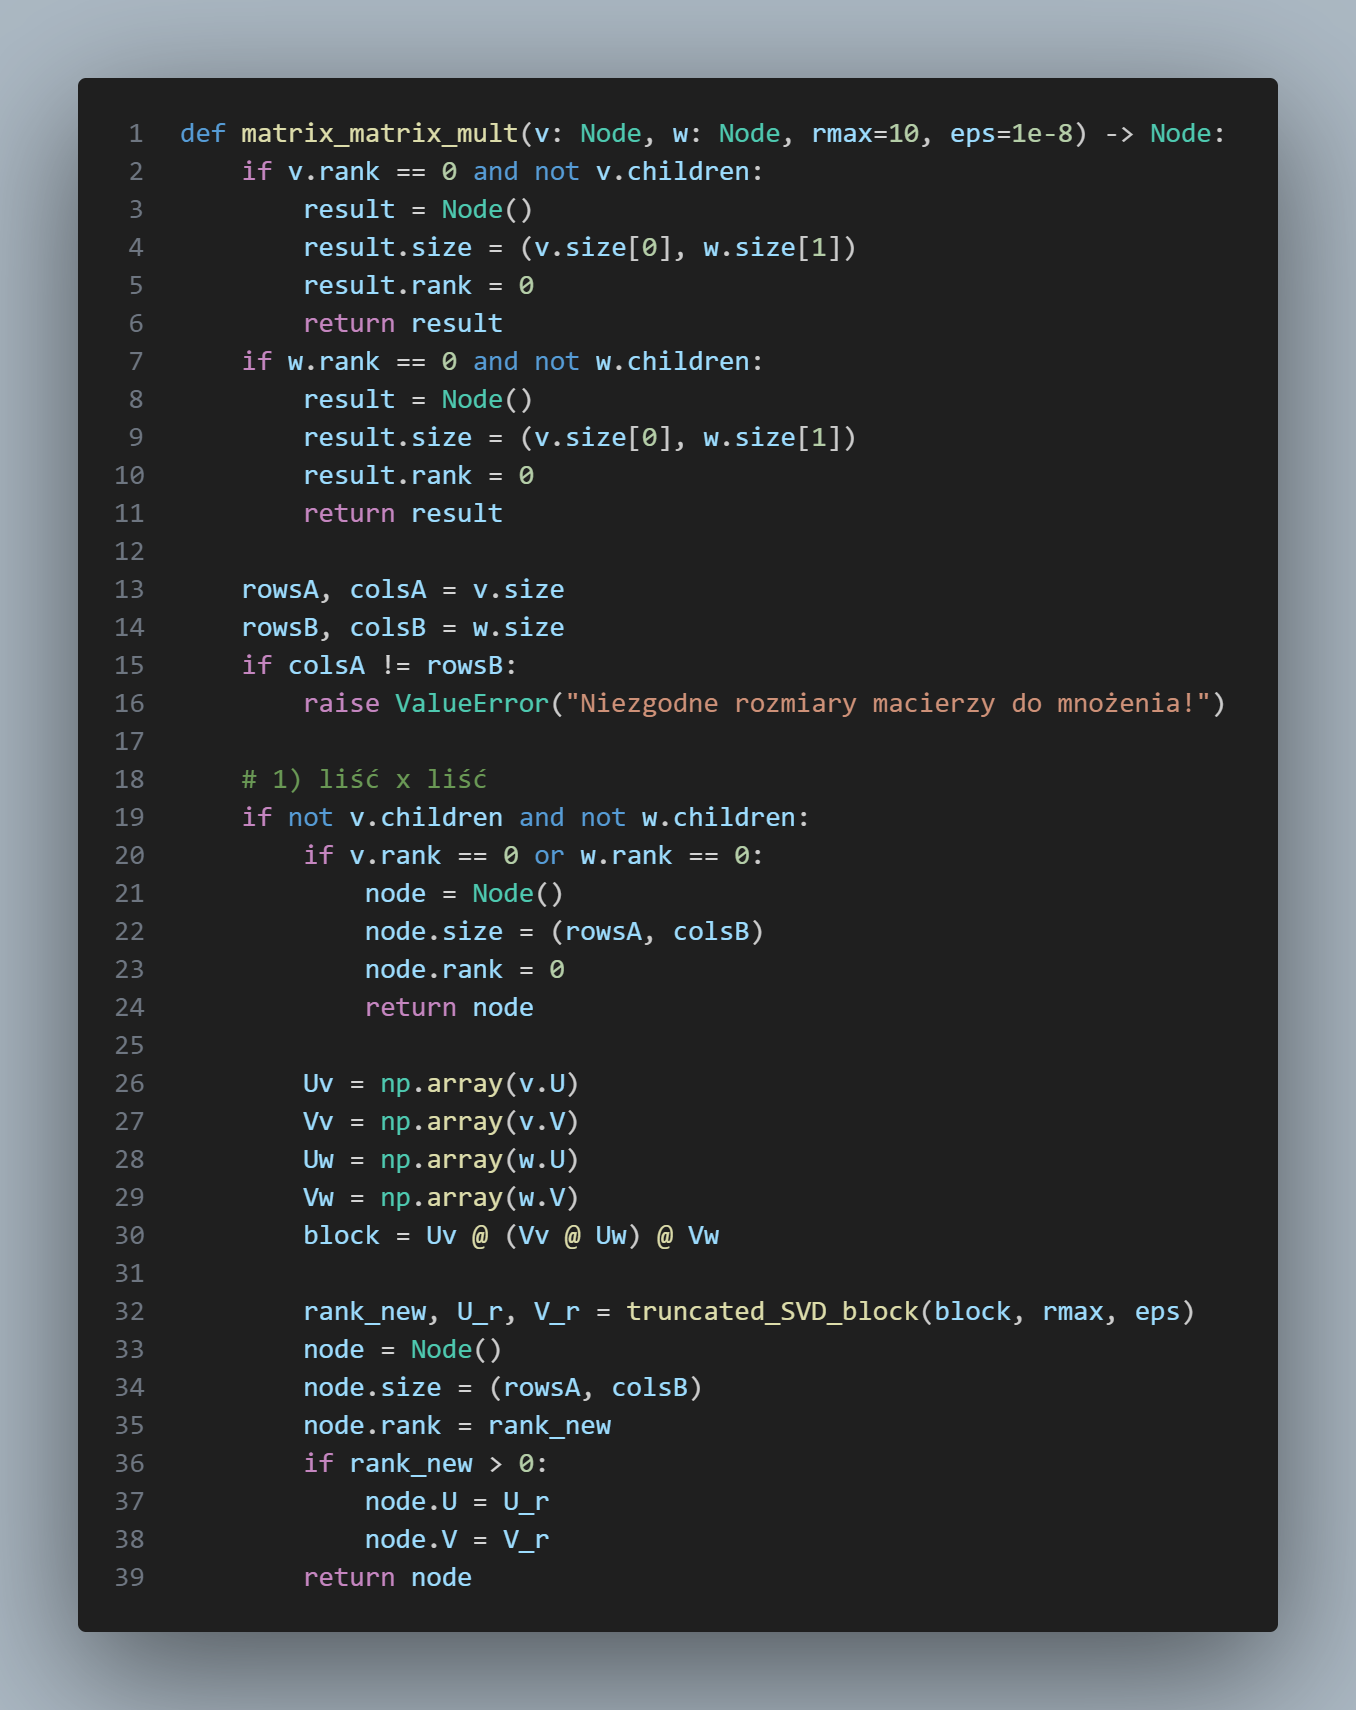
\includegraphics[width=1\linewidth]{matrix_matrix1.png}
        \caption{Mnożenie dwóch macierzy część 1.}
    \end{figure}
    \begin{figure}[H]
        \centering
        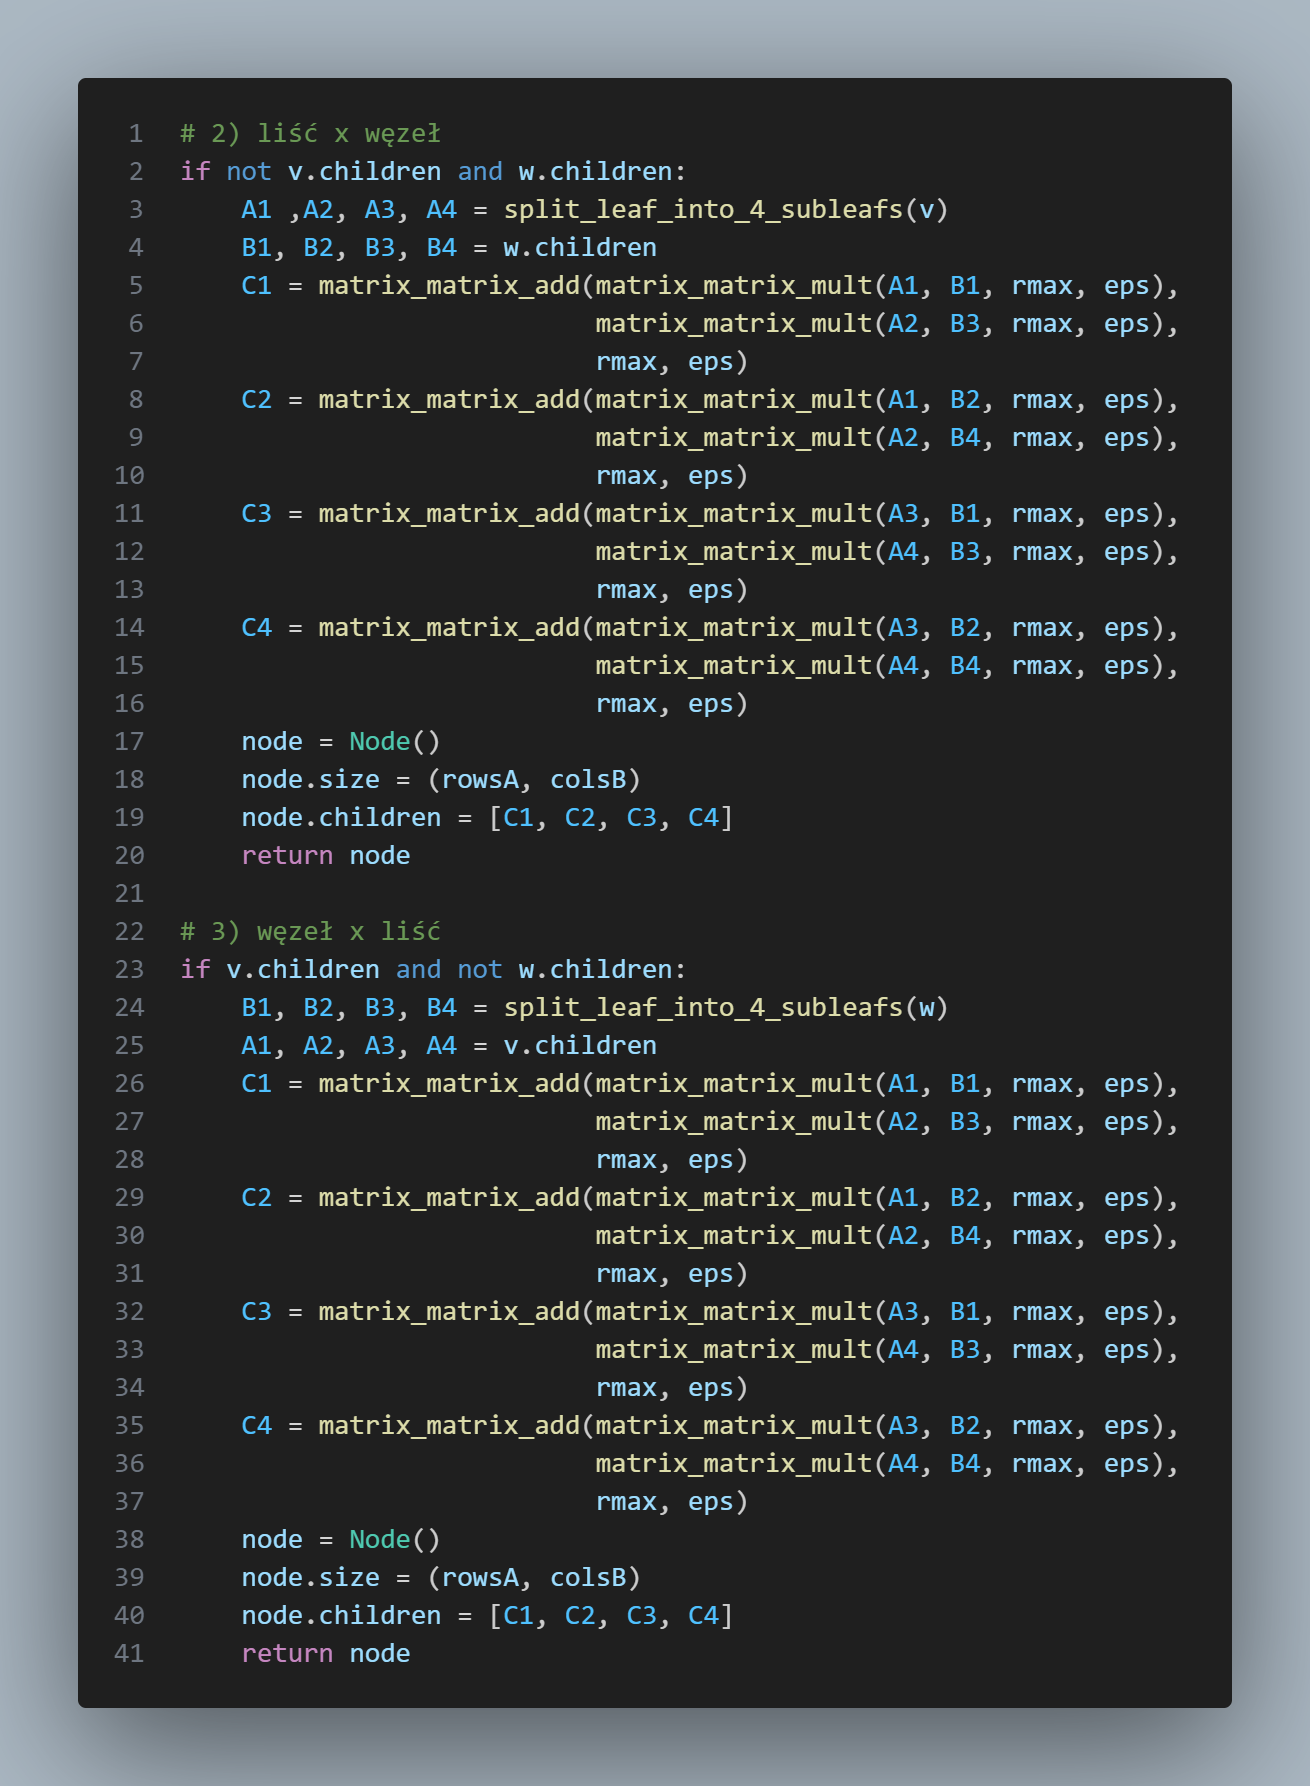
\includegraphics[width=1\linewidth]{matrix_matrix2.png}
        \caption{Mnożenie dwóch macierzy część 2.}
    \end{figure}
    \begin{figure}[H]
        \centering
        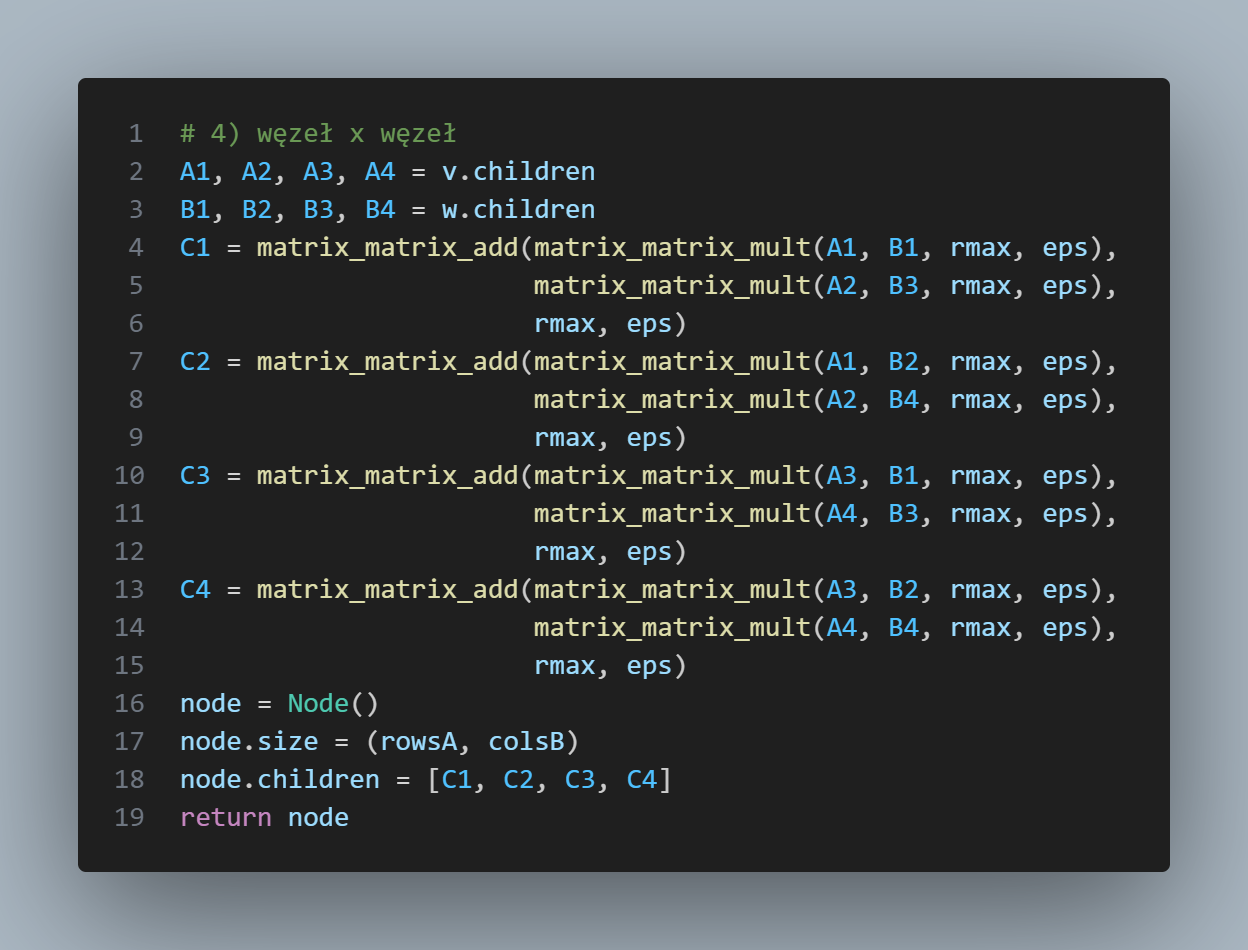
\includegraphics[width=1\linewidth]{matrix_matrix3.png}
        \caption{Mnożenie dwóch macierzy część 3.}
    \end{figure}
    
    \subsection*{}
    Funkcja pomocnicza do mnożenia macierzy:
    \begin{figure}[H]
        \centering
        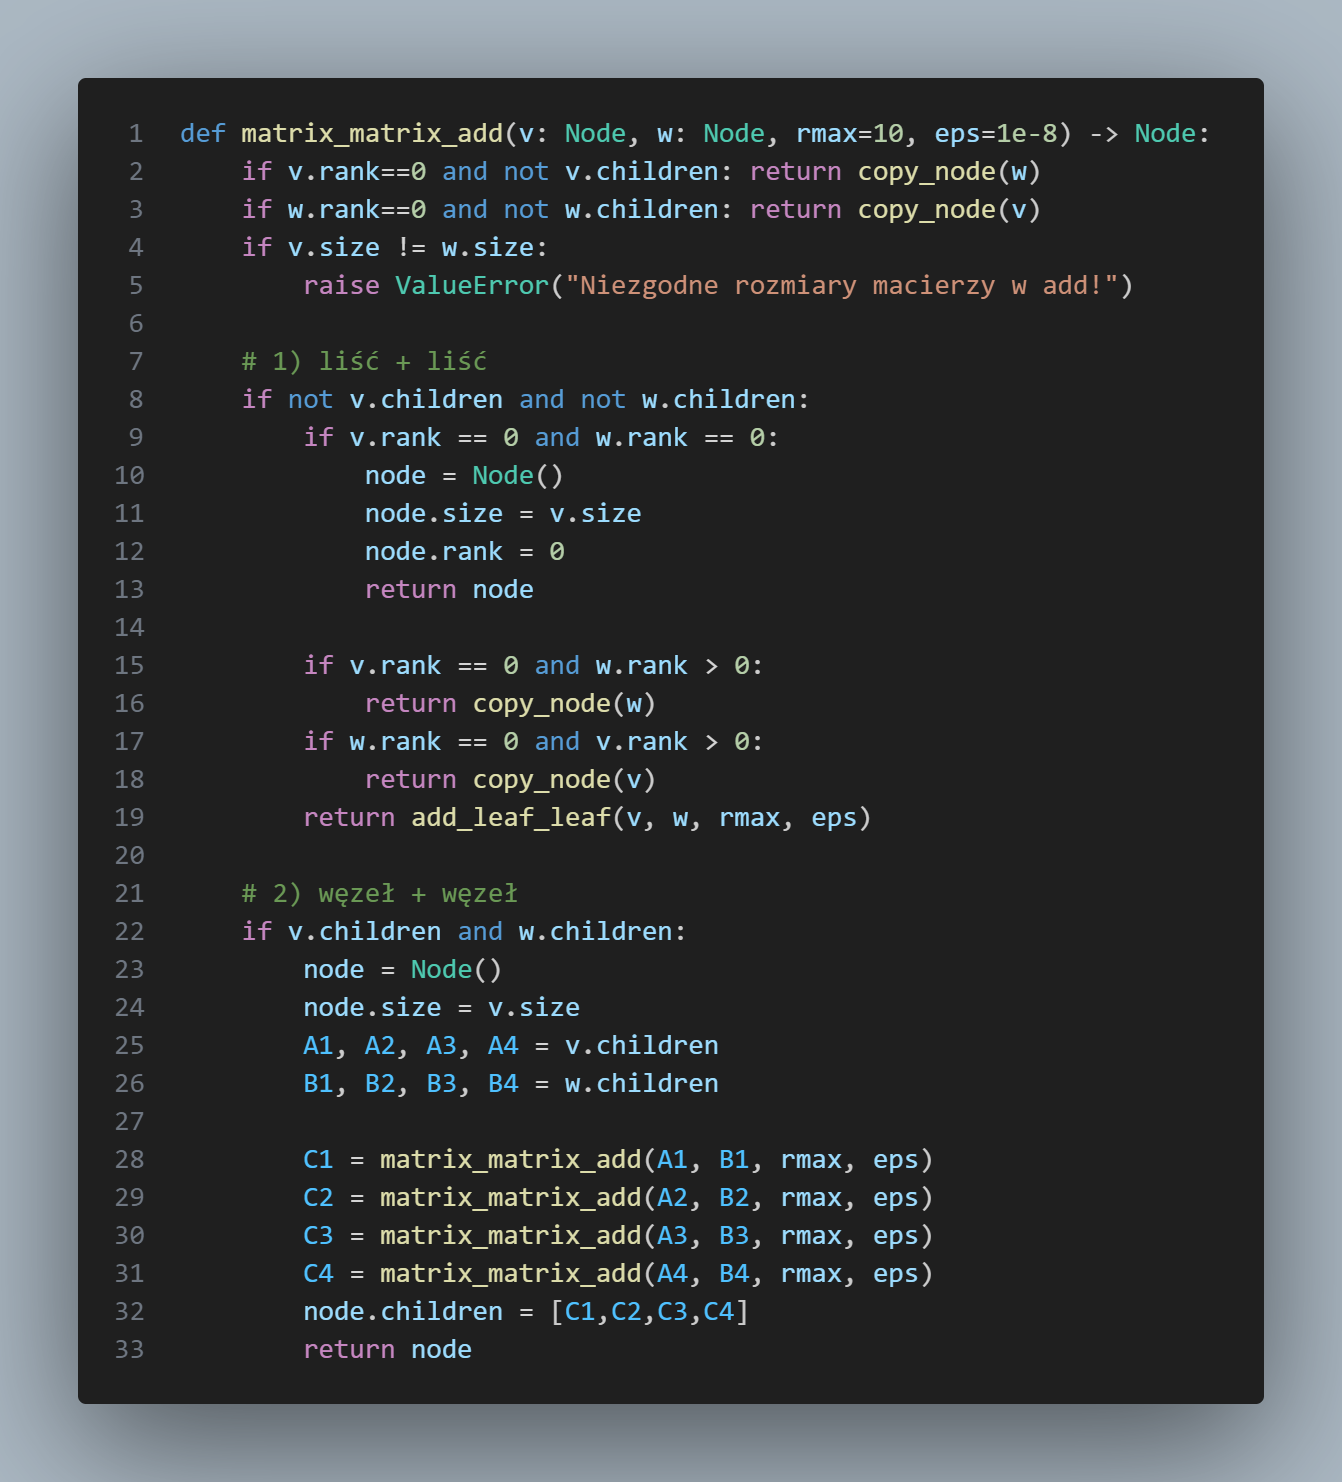
\includegraphics[width=1\linewidth]{matrix_add1.png}
        \caption{Dodawanie część 1.}
    \end{figure}
    \begin{figure}[H]
        \centering
        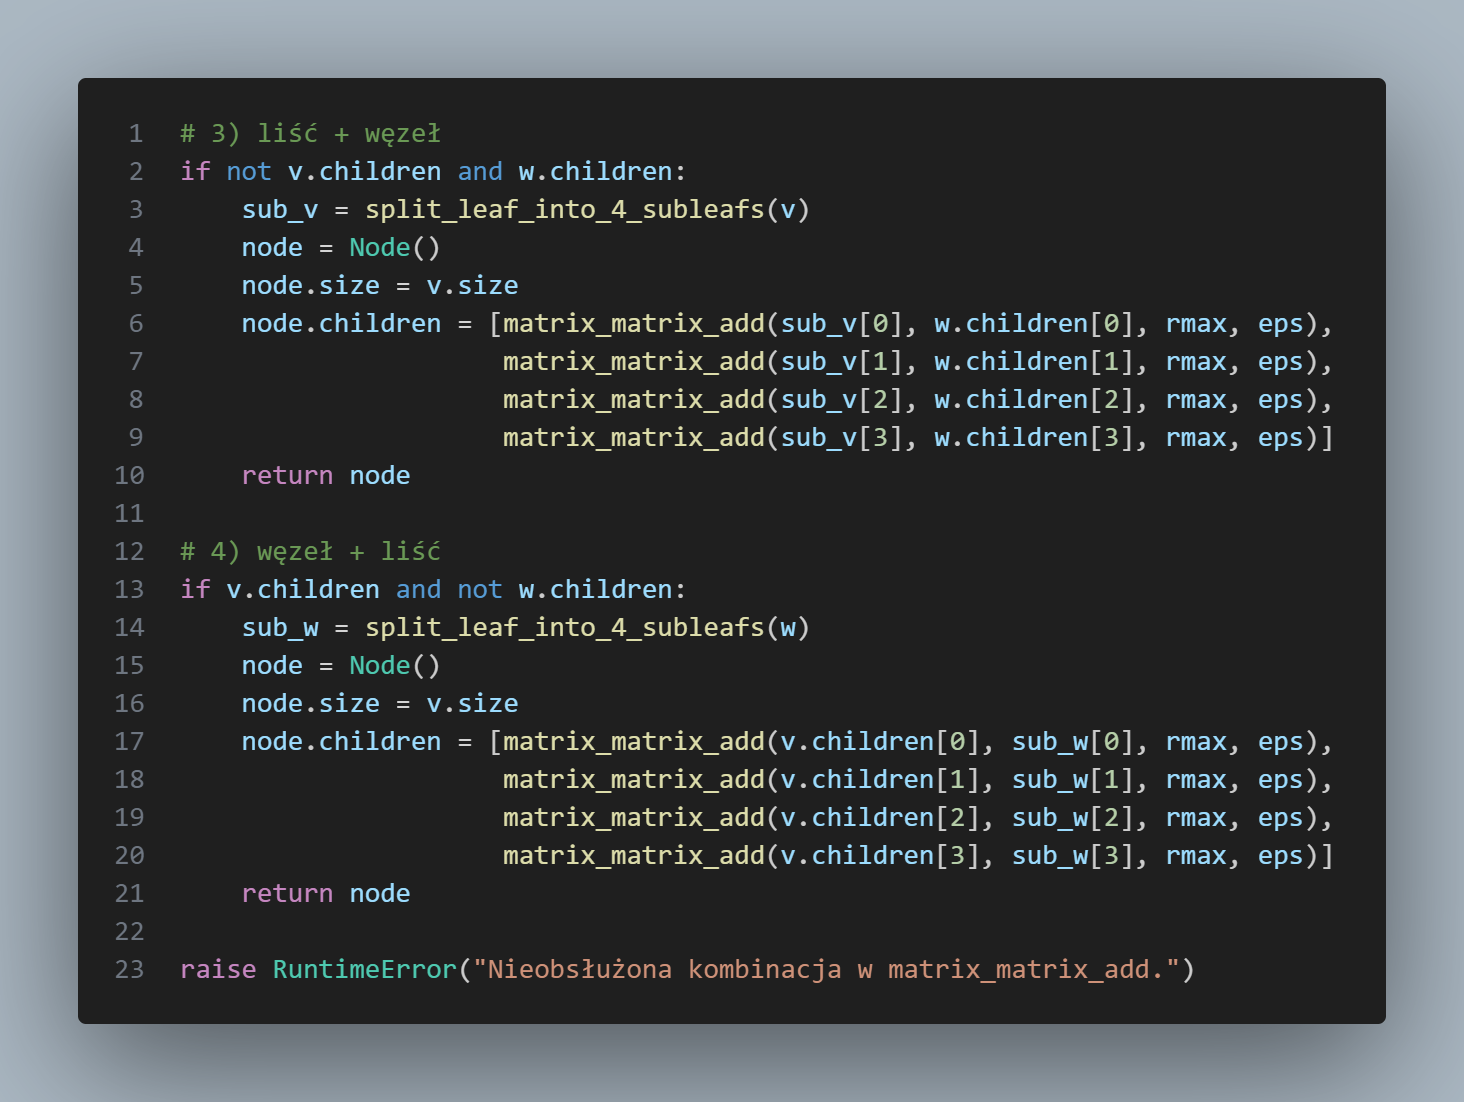
\includegraphics[width=1\linewidth]{matrix_add2.png}
        \caption{Dodawanie część 2.}
    \end{figure}

    \section{Czas działania}
    \begin{figure}[H]
        \centering
        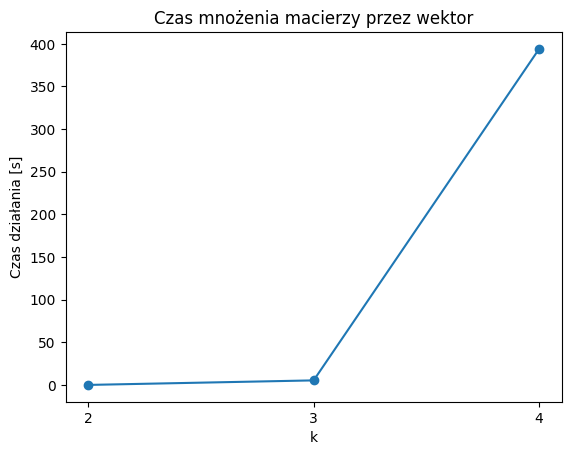
\includegraphics[width=0.7\linewidth]{matrix_vector_time.png}
        \caption{Wykres czasu działania.}
    \end{figure}
    \begin{figure}[H]
        \centering
        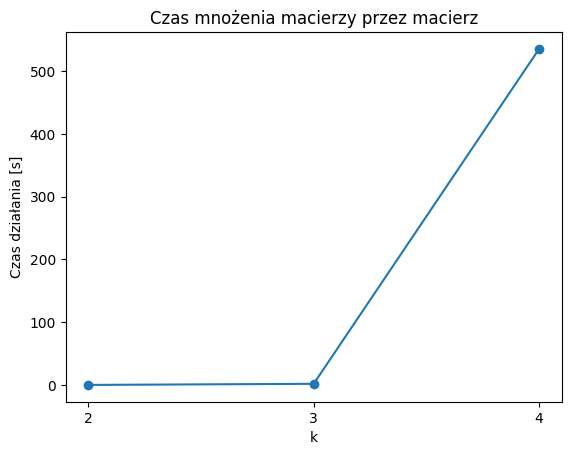
\includegraphics[width=0.7\linewidth]{matrix_matrix_time.png}
        \caption{Wykres czasu działania.}
    \end{figure}

    \section{Oszacowanie złożoności obliczeniowej}
    Do wyników pomiarów, za pomocą funkcji \texttt{curve\_fit}
    z biblioteki \texttt{scipy.optimize}, dopasowana została krzywa
    o równaniu
    \[
        y=\alpha N^\beta
    \]

    \subsection{Mnożenie macierzy i wektora}
    Dopasowana krzywa:
    \[
        y=1,41 \cdot 10^{-5} \cdot N^{2,06}
    \]
    Zatem oszacowana złożoność obliczeniowa wynosi:
    \[
        O(n)=n^{2,06}
    \]
    \begin{figure}[H]
        \centering
        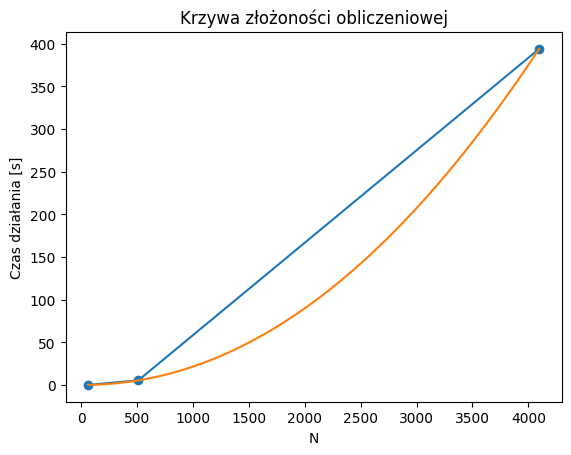
\includegraphics[width=0.7\linewidth]{matrix_vector_comp.png}
        \caption{Krzywa na wykresie.}
    \end{figure}

    \subsection{Mnożenie dwóch macierzy}
    Dopasowana krzywa:
    \[
        y=6,4 \cdot 10^{-8} \cdot N^{2,75}
    \]
    Zatem oszacowana złożoność obliczeniowa wynosi:
    \[
        O(n)=n^{2,75}
    \]
    \begin{figure}[H]
        \centering
        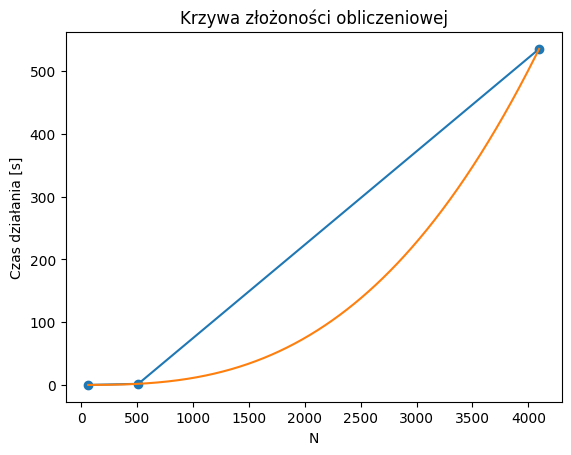
\includegraphics[width=0.7\linewidth]{matrix_matrix_comp.png}
        \caption{Krzywa na wykresie.}
    \end{figure}

    \section{}

\end{document}
